\subsubsection{Módulo Wi-Fi y alimentación USB}


La comunicación del SALT con la central operativa de control se realiza utilizando la red de Internet. Para lograr esa comunicación, se utilizó el módulo ESP32 Devkit-C que tiene la capacidad de conectarse a una red Wi-Fi. Este módulo permite su alimentación con 5V ya que tiene un regulador interno que alimenta el MCU interno con 3V3. La interfaz con el SAL/T se realiza mediante el protocolo UART y se utiliza un pin GPIO para el pin de EN (\textit{enable}) que trae el módulo lo que permite forzar un reset del módulo ante cualquier falla detectada. Para facilitar la programación y el manejo de este módulo, se colocó en la placa principal un zócalo que permita insertar y remover el módulo sin necesidad de soldarlo a la placa. \\




Considerando que la formación puede no tener instalada una red Wi-Fi propia, se consideró la instalación de módulos Wi-Fi - 4G, para poder generar hasta 2 redes Wi-Fi utilizando la red de datos celular. Estos módulos utilizan las tarjetas SIM (\textit{Subscriber Identity Module}); pequeño chip utilizado en dispositivos móviles para identificar de manera única a un usuario en una red de telecomunicaciones que contiene información esencial como el número de teléfono, datos de autenticación y almacenamiento de contactos. Con estos módulos, se puede generar una red Wi-Fi utilizando la red de datos de distintos proveedores de servicio de datos celulares. Existen muchos módulos de estas características y son ampliamente utilizados en la vida cotidiana; por ejemplo, la empresa Altanet cuenta con un módem router Portátil USB 4G LTE Wi-Fi \cite{altanet} que se visualiza en la figura \ref{fig:mod_4g}. Esté módulo trabaja con todas las bandas argentinas incluyendo la banda rural y solo necesita insertarle una tarjeta nano SIM y alimentarlo por USB. 

\begin{figure}[H]
    \centering
    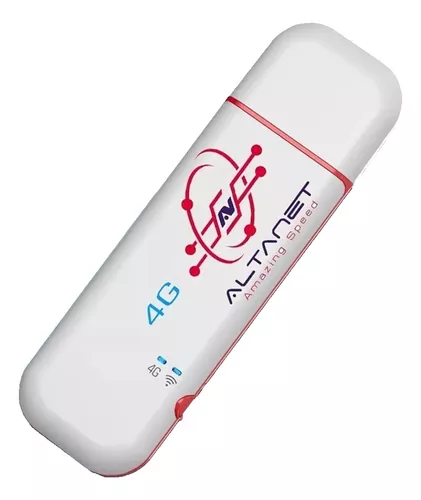
\includegraphics[width = 0.3\linewidth]{img/mod_4g.png}
    \caption{Módem router Portátil USB 4G LTE Wi-Fi de Altanet}
    \label{fig:mod_4g}
\end{figure}    


En el diseño del SAL/T, se colocó en la placa dos conectores USB tipo A del modelo 87583-2010BLF de Amphenol FCI \cite{87583-2010BLF}, con los pines de alimentación conectados a 5V. Estos conectores están pensados para alimentar estos módulos Wi-Fi - 4G. Los módulos Wi-Fi -4G no fueron incluidos en el prototipo por su costo y por su fácil reemplazo por cualquier red Wi-fi generada por un router o teléfono para realizar las pruebas del sistema. 
